\documentclass[11pt,twoside]{article}
 \usepackage{nopageno}
\usepackage{pdfpages}

%FAQ
\usepackage{lipsum}
\newcounter{question}
\setcounter{question}{0}

\usepackage[section]{placeins}

% bibliography
\usepackage[numbers]{natbib}

% MATLAB code package
\usepackage{listings}
\usepackage[framed]{matlab-prettifier}
\usepackage[T1]{fontenc}
\definecolor{light-gray}{gray}{0.95}
\definecolor{matlab-yellow}{RGB}{252,251,220}

\usepackage{upquote}
\usepackage{xspace}
\usepackage{graphicx}

\usepackage{todonotes}
\usepackage{microtype}


% For math symbol, equations, etc...
\RequirePackage{amsmath}
\RequirePackage{amsfonts}
\RequirePackage{amssymb}
\RequirePackage{latexsym}
\RequirePackage{amscd}
\RequirePackage{mathtools}
\RequirePackage{bm}

\usepackage{mathabx}

\usepackage{hyperref}
\hypersetup{colorlinks=true,linkcolor=blue}

\usepackage{subcaption} 
\usepackage[capitalise,noabbrev]{cleveref}

% For table
\usepackage{booktabs}
\usepackage{multirow}
\usepackage{array}
\newcommand{\xbar}[1]{\overline{#1}}
\newcolumntype{L}[1]{>{\raggedright\arraybackslash}m{#1}} 
\newcolumntype{C}[1]{>{\centering\arraybackslash}m{#1}} 
\newcolumntype{R}[1]{>{\raggedleft\arraybackslash}m{#1}} 
\newcolumntype{N}{@{}m{0pt}@{}}

% For description
\usepackage{enumitem}
\setlist[description]{%
  topsep=30pt,               % space before start / after end of list
  itemsep=5pt,               % space between items
  font={\normalfont\textbullet\space}, % set the label font
}

% For rotating figures, tables, etc.  including their captions
\usepackage[figureleft]{rotating}

%%%%%%%%%%%%%%%%%%%%%%%%%%%%
%TIKZ PACKAGE
%%%%%%%%%%%%%%%%%%%%%%%%%%%%
\usepackage{tikz}
\usetikzlibrary{calc,patterns,decorations.pathmorphing,decorations.markings,decorations.pathreplacing}
\usetikzlibrary{shapes,fit}
\usetikzlibrary{positioning}
\usetikzlibrary{matrix}
\usetikzlibrary{decorations.text}
%\usetikzlibrary{decorations.markings}
\usetikzlibrary{shapes.geometric,arrows,positioning}
\usetikzlibrary{positioning,arrows.meta,bending}
%Rectangle
\tikzstyle{rect}=[rectangle, minimum width=2.2cm,minimum height=1.2cm,draw=black!100, thick]
\tikzstyle{wrect}=[rectangle, minimum width=2.2cm,minimum height=1.2cm,draw=white!100, thick]
\tikzstyle{smallrect}=[rectangle, minimum width=1cm,minimum height=0.5cm,draw=black!100, thick]
\tikzstyle{smallrectm}=[rectangle, minimum width=1.5cm,minimum height=0.5cm,draw=black!100, thick]
\tikzstyle{PCA}=[rectangle, minimum width=2.2cm,minimum height=1.2cm,draw=red!100, very thick,rounded corners]
\tikzstyle{user}=[circle,draw, inner sep = 1.5pt]
\tikzstyle{eslightgray}=[rectangle, draw=black!100, thick,fill opacity=0.5, text opacity=1, fill=lightgray, minimum height = 1cm, inner sep=0pt]
\tikzstyle{esaliceblue}=[rectangle, draw=black!100, thick, fill=aliceblue, minimum height = 1cm, inner sep=0pt]
\tikzstyle{esbabyblueeyes}=[rectangle, draw=black!100, thick, fill=babyblueeyes, minimum height = 1cm, inner sep=0pt]
\tikzstyle{esbabyblueeyestransp}=[rectangle, draw=black!100, thick fill=babyblueeyes, fill opacity=0.2, text opacity=1,  minimum height = 1cm, inner sep=0pt]
\tikzstyle{esbisque}=[rectangle, draw=black!100, thick, fill=bisque, minimum height = 1cm, inner sep=0pt, fill opacity=0.5, text opacity=1]
\tikzstyle{esbisquetransp}=[rectangle, draw=black!100, thick, fill=bisque, fill opacity=0.5, text opacity=1, minimum height = 1cm, inner sep=0pt]
\tikzstyle{esceladon}=[rectangle, draw=black!100, thick, fill=celadon, minimum height = 1cm, inner sep=0pt]
\tikzstyle{eswhite}=[rectangle, draw=black!100, thick, fill=white, minimum height = 1cm, inner sep=0pt, draw=black!100, thick]
\tikzstyle{esamber}=[rectangle, draw=black!100, thick, fill=amber, minimum height = 1cm, inner sep=0pt, draw=black!100,  thick]
\tikzstyle{esbrightlavender}=[rectangle, draw=black!100, thick, fill=brightlavender, minimum height = 1cm, inner sep=0pt, draw=black!100,  thick]
\tikzstyle{para}=[trapezium ,minimum height=0.8 cm, draw=black!100, thick, trapezium left angle=-120, trapezium right angle=-60,trapezium stretches, inner sep = 0pt]
\tikzstyle{paraamber}=[trapezium , fill=amber, minimum height=0.8 cm, draw=black!100, thick, trapezium left angle=-120, trapezium right angle=-60,trapezium stretches, inner sep = 0pt]
\tikzstyle{parababyblueeyes}=[trapezium , fill=babyblueeyes, minimum height=0.8 cm, draw=black!100, thick, trapezium left angle=-120, trapezium right angle=-60,trapezium stretches, inner sep = 0pt]
\tikzstyle{paraambertransp}=[trapezium , fill=amber, minimum height=0.8 cm, draw=black!100, thick, fill opacity=0.2, text opacity=1, trapezium left angle=-120, trapezium right angle=-60,trapezium stretches, inner sep = 0pt]
\tikzstyle{paraceladon}=[trapezium , fill=celadon, minimum height=0.8 cm, draw=black!100, thick, trapezium left angle=-120, trapezium right angle=-60,trapezium stretches, inner sep = 0pt]
\tikzstyle{parabisque}=[trapezium , fill=bisque, minimum height=0.8 cm, draw=black!100, thick,  fill opacity=0.5, text opacity=1, trapezium left angle=-120, trapezium right angle=-60,trapezium stretches, inner sep = 0pt]
\tikzstyle{paralightgray}=[trapezium , fill=lightgray, minimum height=0.8 cm, draw=black!100, thick,  fill opacity=0.5, text opacity=1, trapezium left angle=-120, trapezium right angle=-60,trapezium stretches, inner sep = 0pt]
\tikzstyle{parawhite}=[trapezium , fill=white, minimum height=0.8 cm, draw=black!100, thick,  fill opacity=0.5, text opacity=1, trapezium left angle=-120, trapezium right angle=-60,trapezium stretches, inner sep = 0pt]

% Parallelogram
\tikzstyle{para}=[trapezium, minimum width=3cm,minimum height=1.2cm, draw=black!100,  thick, trapezium left angle=-150, trapezium right angle=-30,trapezium stretches]
%Hexagone in text
\tikzstyle{hexa}=[signal, signal to=left and right, minimum width=4cm,minimum height=1.2cm, draw=black!100, thick]

 \tikzstyle{user}=[circle,draw, inner sep = 1.5pt]
 \tikzstyle{test}=[diamond, aspect=1, minimum width=1.5cm, minimum height = 1.5cm, draw=black!100, thick,  inner sep=-1pt]
 \tikzstyle{testamber}=[diamond, fill=amber, aspect=1, minimum width=1.5cm, minimum height = 1.5cm, draw=black!100, thick,  inner sep=-1pt]
 \tikzstyle{testbabyblueeyes}=[diamond, fill=babyblueeyes, aspect=1, minimum width=1.5cm, minimum height = 1.5cm, draw=black!100, thick,  inner sep=-1pt]
 \tikzstyle{testbisque}=[diamond, fill=bisque, aspect=1, minimum width=1.5cm, minimum height = 1.5cm, draw=black!100, thick,  inner sep=-1pt, fill opacity=0.5, text opacity=1]
 \tikzstyle{testceladon}=[diamond, fill=celadon, aspect=1, minimum width=1.5cm, minimum height = 1.5cm, draw=black!100, thick,  inner sep=-1pt]
 \tikzstyle{testlightgray}=[diamond, fill=lightgray, aspect=1, minimum width=1.5cm, minimum height = 1.5cm, fill opacity=0.5, text opacity=1, draw=black!100, thick,  inner sep=-1pt]
  \tikzstyle{testwhite}=[diamond, fill=white, aspect=1, minimum width=1.5cm, minimum height = 1.5cm, draw=black!100, thick,  inner sep=-1pt]
 
%Connecting link
\tikzstyle{connect}=[-latex, thick,>=latex]
\tikzstyle{shaded}=[draw=black!20,fill=black!20]
\tikzstyle{line} = [draw, -latex,thick,>=latex]

\definecolor{egg}{RGB}{250,250,235}
\definecolor{aliceblue}{rgb}{0.94, 0.97, 1.0}
\definecolor{babyblueeyes}{rgb}{0.63, 0.79, 0.95}
\definecolor{bisque}{rgb}{0.91, 0.45, 0.32}
\definecolor{celadon}{rgb}{0.67, 0.88, 0.69}
\definecolor{amber}{rgb}{1.0, 0.99, 0.82}%{1.0, 0.75, 0.0}
\definecolor{brightlavender}{rgb}{0.75, 0.58, 0.89}

\graphicspath{{./docfigs/}}


\title{
\includegraphics[width=100mm]{OpenBDLM_logo.pdf}\\[20pt]
 OpenBDLM V1.0 reference manual}
\author{Ianis Gaudot, Luong H. Nguyen, James-A. Goulet \\ Polytechnique Montreal}

\begin{document}

\newcommand{\MATLAB}{\textsc{Matlab}}




 \begin{lstlisting}[ frame = single, basicstyle = \mlttfamily \small, label = LST:OpenBDLMStartingMenuExample1, linewidth=\linewidth, captionpos=b]
>> [data, model, estimation, misc] = OpenBDLM_main;

------------------------------------------------
     Starting OpenBDLM_V1.0
------------------------------------------------
            Time series analysis using 
            Bayesian Dynamic Linear Models
------------------------------------------------
- Start a new project: 

     *      Enter a configuration filename 
     0   -> Interactive tool 

- Type D to Delete project(s), V for Version control, Q to Quit.

     choice >> 0
     
---------------------------------------
          Starting a new project...
----------------------------------------

- Enter a project name (max 25 characters):
     choice >> Example_DISP
     
- Does this project aim to create synthetic data ? (y/n) 
     choice >> no

     Load data...

- Choose a database

     0   -> Build a new database     	
 
     choice >> 0
     
- Data available: 
 
     Time series number #      Reference name            Size                     	
     -----------------------------------------------------------------
     1                         DISP                      [19366x1]                	
     -----------------------------------------------------------------
        
     - How many model classes do you want for each time-series? 
     choice >> 1
     
     --------------------------------------------------------
     BDLM Component reference numbers
     --------------------------------------------------------
     11: Local level 
     12: Local trend 
     13: Local acceleration 
     21: Local level compatible with local trend 
     22: Local level compatible with local acceleration 
     23: Local trend compatible with local acceleration 
     31: Periodic 
     41: Autoregressive process (AR(1)) 
     51: Kernel regression 
     61: Level Intervention 
     --------------------------------------------------------

- Identify components for time series #1; e.g. [11 31 41]
     choice >> [11 31 31 41]

     Building model...
     Saving project...
     Project saved in saved_projects/PROJ_Example_DISP.mat. 
     Printing configuration file...
     Saving data...

     Database saved in data/mat/DATA_Example_DISP.mat 
     Configuration file saved in config_files/CFG_Example_DISP.m. 
     
     
     ----------------------------------------------- 
/    OpenBDLM main menu. Choose from
----------------------------------------------------

     1  ->  Learn model parameters values 
     2  ->  Estimate initial hidden states values 
     3  ->  Estimate hidden states values 

     11 ->  Display and modify current model parameter values 
     12 ->  Display and modify current initial hidden states values 
     13 ->  Display and modify current training period 
     14 ->  Plots 
     15 ->  Display model matrices 
     16 ->  Create synthetic data 
     17 ->  Export
     18 ->  Display current options in configuration file format 

     Type Q to Save and Quit 

     choice >> 1
     
---------------------------------------------
/ Learn model parameters
--------------------------------------------

     1 ->  Newton-Raphson
     2 ->  Stochastic Gradient Ascent

     Type R to return to the previous menu

     choice >> 1

     Learning model parameters (Newton-Raphson) ...

    \Start Newton-Raphson maximization  algorithm 
    (finite difference method)

      Training period:                                    1-Inf [days]
      Maximal number of iteration:                        3
      Total time limit for calibration :                  60 [min]
      Convergence criterion:                              1e-07*LL
      Nb. of search levels for \lambda:                   4*2

           Initial LL: 36627.6547
                       AR|M1|1         AR|M1|1         |M1|1            
      parameter names: \phi            \sigma_w        \sigma_v         
       initial values: +7.50e-01       +1.74e-02       +8.70e-03       
--------------------------
    Loop #1 : AR|M1|1 | \sigma_w 
       delta_param: 0.0048527 
    log-likelihood : 40472.2846
    param change   : 0.0174 -> 0.022253

                    AR|M1|1         AR|M1|1         |M1|1           
   parameter names: \phi            \sigma_w        \sigma_v        
    current values: +7.50e-01       +2.23e-02       +8.70e-03      
  current f.o. std: +0.00e+00       +5.63e-05       +0.00e+00      
      previous dLL: +1.00e+06       +3.84e+03       +1.00e+06      
         converged: +0.00e+00       +0.00e+00       +0.00e+00      

--------------------------
    Loop #2 : AR|M1|1 | \phi 
       delta_param: 0.16243 
    log-likelihood : 46976.3494
    param change   : 0.75 -> 0.91243

                    AR|M1|1         AR|M1|1         |M1|1           
   parameter names: \phi            \sigma_w        \sigma_v        
    current values: +9.12e-01       +2.23e-02       +8.70e-03      
  current f.o. std: +1.94e-03       +5.63e-05       +0.00e+00      
      previous dLL: +6.50e+03       +3.84e+03       +1.00e+06      
         converged: +0.00e+00       +0.00e+00       +0.00e+00      

--------------------------
    Loop #3 : |M1|1 | \sigma_v 
       delta_param: -0.0056165 
    log-likelihood : 47795.5556
    param change   : 0.0087002 -> 0.0030837

                    AR|M1|1         AR|M1|1         |M1|1           
   parameter names: \phi            \sigma_w        \sigma_v        
    current values: +9.12e-01       +2.23e-02       +3.08e-03      
  current f.o. std: +1.94e-03       +5.63e-05       +2.02e-04      
      previous dLL: +6.50e+03       +3.84e+03       +8.19e+02      
         converged: +0.00e+00       +0.00e+00       +0.00e+00      

          Warning: the optimization has reached the  
          maximum number of loops (3) without convergence 

 ----------------------
    Final results
 ----------------------
   log-likelihood: 47795.5556
                   AR|M1|1         AR|M1|1         |M1|1           
  parameter names: \phi            \sigma_w        \sigma_v        
   current values: +9.12e-01       +2.23e-02       +3.08e-03      
 current f.o. std: +1.94e-03       +5.63e-05       +2.02e-04      

----------------------------------------------- 
/     OpenBDLM main menu. Choose from 
-----------------------------------------------

     choice >>  2
         
 --------------------------------------------------
 /    OpenBDLM main menu. Choose from 
-------------------------------------------------- 

     choice >> 3

----------------------------------------------------
/    State estimation
----------------------------------------------------

     1 ->  Filter 
     2 ->  Smoother 

     Type R to return to the previous menu 

     choice >> 1

-------------------------------------------------------
/    OpenBDLM main menu. Choose from 
------------------------------------------------------- 

     choice >> 17

-------------------------------------------------------
/    Export menu
------------------------------------------------------

     1 ->  Export the project in a configuration file
     2 ->  Export data in CSV format
     3 ->  Export results in CSV format
     4 ->  Create and export figures 

     Type R to return to the previous menu

     choice >> 1
     Printing configuration file...
     Saving data...
     Database saved in data/mat/DATA_Example_DISP.mat
     Configuration file saved in config_files/CFG_Example_DISP.m.
     
 ----------------------------------------------------
/    OpenBDLM main menu. Choose from 
---------------------------------------------------- 

     choice >> Q  
     
\end{lstlisting}


%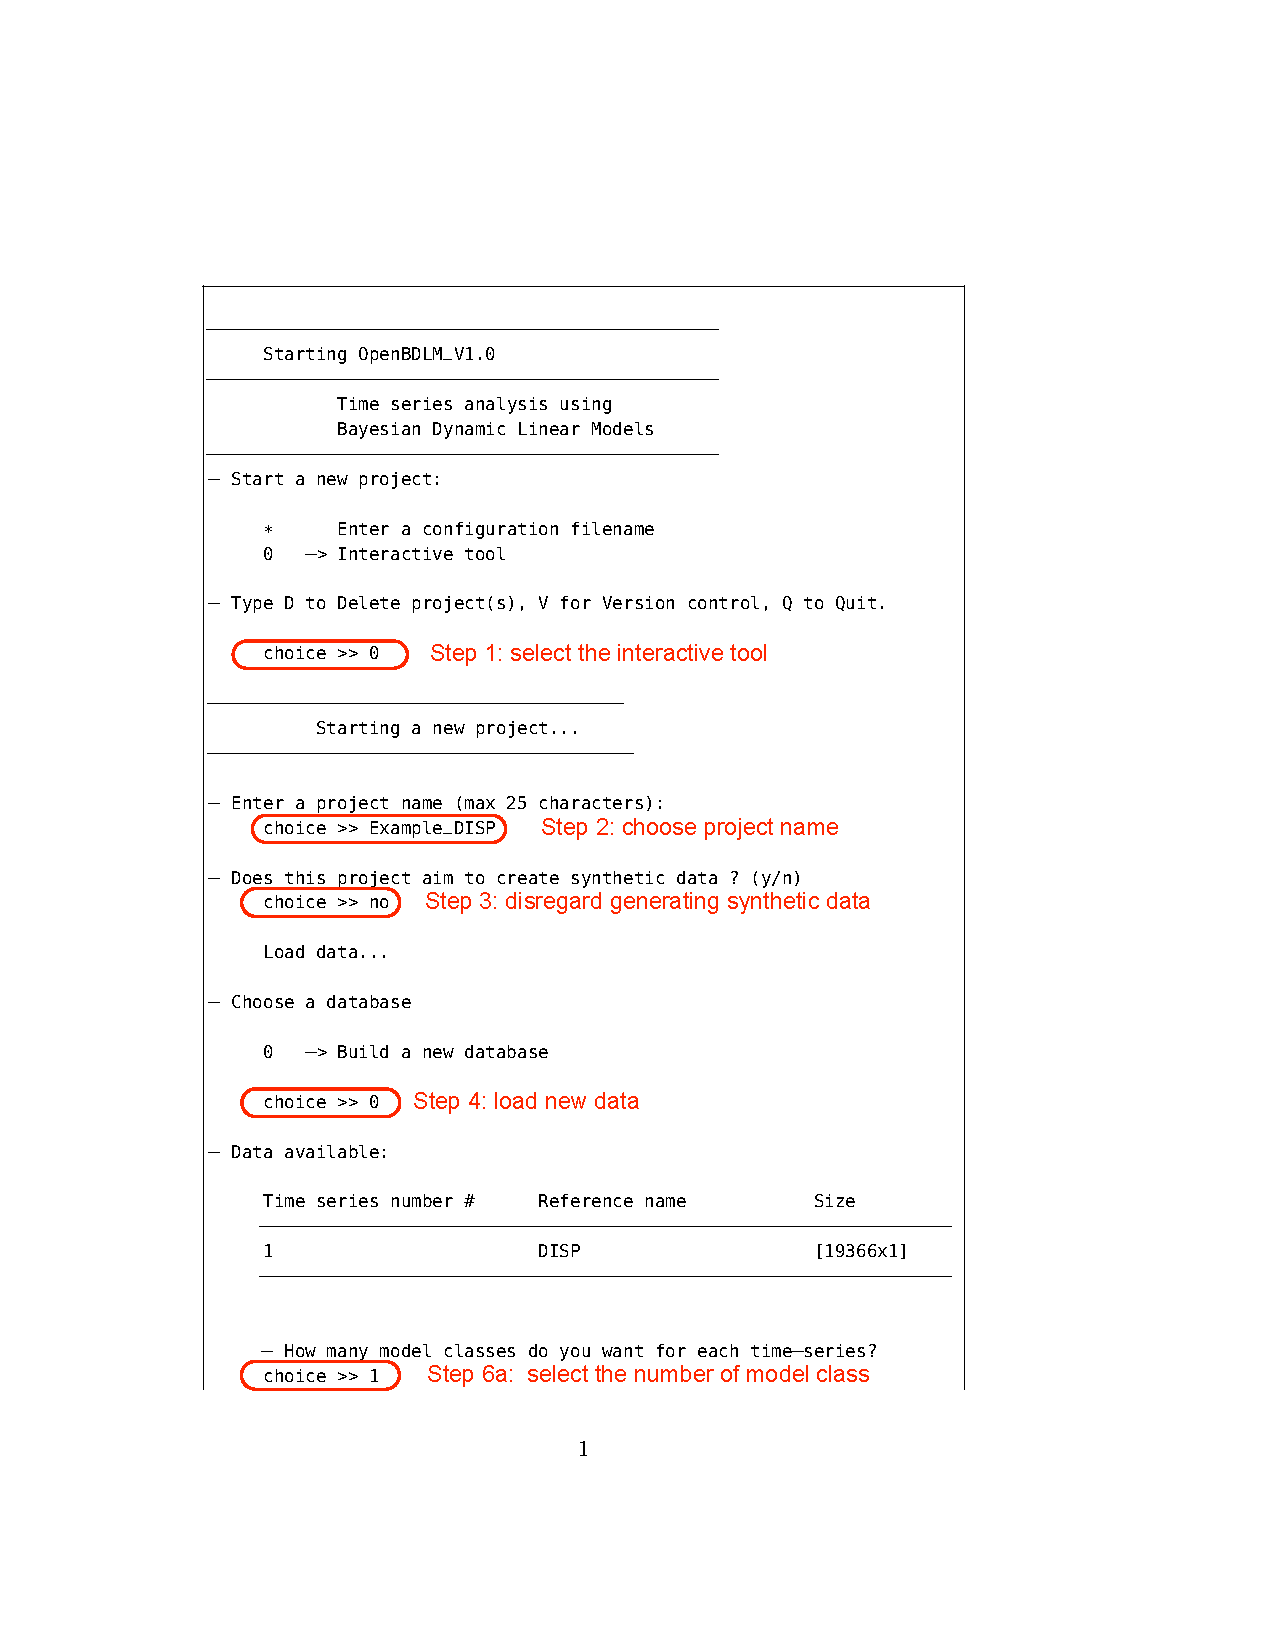
\includepdf[pages=-, pagecommand={\thispagestyle{plain}}]{test.pdf}


\end{document}

